%A classe é a dcc-nce, e o parâmetro a ser informado é diss (para dissertação de mestrado)
\documentclass[diss]{dcc-nce}
\usepackage[T1]{fontenc}
\usepackage{color,graphicx}
\usepackage{graphics}
\usepackage{url}
\usepackage{amsmath,amssymb}
%\usepackage[numbers]{natbib}
\usepackage{natbib}
\usepackage{dsfont} %Usado para conjuntos N, Z, Q, R, C
\usepackage[portuguese,algoruled,longend]{algorithm2e}
\usepackage{algorithmic}
\usepackage[utf8]{inputenc}
\usepackage{listings}%Para inserir codigos fontes de programas no apendice.
\usepackage{xcolor}
% Definindo novas cores
\definecolor{verde}{rgb}{0,0.5,0}
% Configurando layout para mostrar codigos C++
\usepackage{listings}
\lstset{
  language=C++,
  basicstyle=\ttfamily\small,
  keywordstyle=\color{blue},
  stringstyle=\color{verde},
  commentstyle=\color{red},
  extendedchars=true,
  showspaces=false,
  showstringspaces=false,
  numbers=left,
  numberstyle=\tiny,
  breaklines=true,
  backgroundcolor=\color{green!10},
  breakautoindent=true,
  captionpos=b,
  xleftmargin=0pt,
}

% Para contagem do numero total de folhas:
\usepackage{everyshi}
\makeatletter
\let\totalpages\relax
\newcounter{mypage}
\EveryShipout{\stepcounter{mypage}}
\AtEndDocument{\clearpage
   \immediate\write\@auxout{%
    \string\gdef\string\totalpages{\themypage}}}
\makeatother


\topmargin=0in
\textheight=20.5cm


\begin{document}

%Este tem que vir primeiro neste arquivo, caso contrario nao aparecerao
%as palavras-chave na ficha catalografica:
\keyword{Palavra-chave 1}
\keyword{Palavra-chave 2}
\keyword{Palavra-chave 3}

\cip{}


    % Editar o arquivo palavrasChavePortugues

%O restante vem depois:
\title{Coloque aqui o título da sua dissertação}

% COLOCAR AQUI O CUTTER (CÓDIGO FORNECIDO PELA BIBLIOTECA DO NCE PARA A FICHA CATALOGRÁFICA):
\codigobiblioteca{CBIB}

\author{Último Sobrenome do Aluno}{Nome Sobrenome1 Sobrenome2 ...}
\advisor[Prof.~Dr.~]{Último Sobrenome}{Nome Sobrenome1 Sobrenome2 ...}
\coadvisor[Profa. Dra.]{Último Sobrenome}{Nome Sobrenome1 Sobrenome2 ...}
\banca{Profa. Dr. Fulano de Tal}{Prof. Dr. Beltrano}{Prof. Dr. Ciclano}
\date{2006}
\maketitle
                      % Editar o arquivo capa.tex
\pagenumbering{roman} %numeração de páginas em romano começa a partir do primeiro capítulo

\clearpage

\mbox{}\vfill

\begin{flushright}

{\sffamily\itshape

Aqui coloque a dedicatória...

Se não houver, delete esta parte.

}

\end{flushright}
               % Editar o arquivo dedicatoria.tex
\begin{agradecimentos}
Coloque aqui os agradecimentos.

Agradeço aos meus pais, meu orientador, à bolsa, etc...
\end{agradecimentos}
            % Editar o arquivo agradecimentos.tex
\begin{abstract}

%MADUREIRA, Rodrigo Lopes Rangel. Algoritmos de interseções, bla bla bla...\\

Resumo em português.

\end{abstract}
           % Editar o arquivo resumoPortugues.tex
\begin{englishabstract}{}{coloque aqui as palavras-chave em inglês, separadas por vírgula}

Colocar aqui o resumo em inglês.
\end{englishabstract}

              % Editar o arquivo resumoIngles.tex

\listoffigures{}

\listoftables{}

%% Examples

\begin{listofabbrv}{XXXXXX}
  \item [BCNF] Boyce Codd Normal Form
  \item [XSLT] XSL Transformations
\end{listofabbrv}
    % Editar o arquivo listaAbreviaturaSiglas.tex

\tableofcontents{}                  % Sumário

\parindent=1.25cm %start for each paragraph from the left margin
\parskip=20pt
\baselineskip=20pt


\chapter{Introdução}

Aqui é a introdução da dissertação.

Vamos fazer algumas referências bibliográficas. O estilo a ser usado é o ABNT.

%Este é um relatório técnico \cite{BON03}, um livro \cite{SILBERSCHATZ}, um relatório técnico \cite{PIERCE}, referência da Web \cite{DB2XML}, trabalho de final de curso \cite{Angelo}, e tese de doutorado \cite{HAR98}.

%Artigo sem ano \citet{SPH03}.
%Artigo sem ano \citet{SPH03}.  \\
Artigo sem ano \citet{Longuet-1950}.   \\
%\citet{Hou95} \\
%\citeauthor{Hou95} \\
%\citeonline{Hou95}
Em \citep{SPH_LIU_2003}
Em \cite{Scan-1990-Blelloch}

\section{Motivação}

Uma seção...

Agora vamos referenciar a Figura \ref{figuraEPS}.

\begin{figure}
   \begin{center}
     \scalebox{0.5}{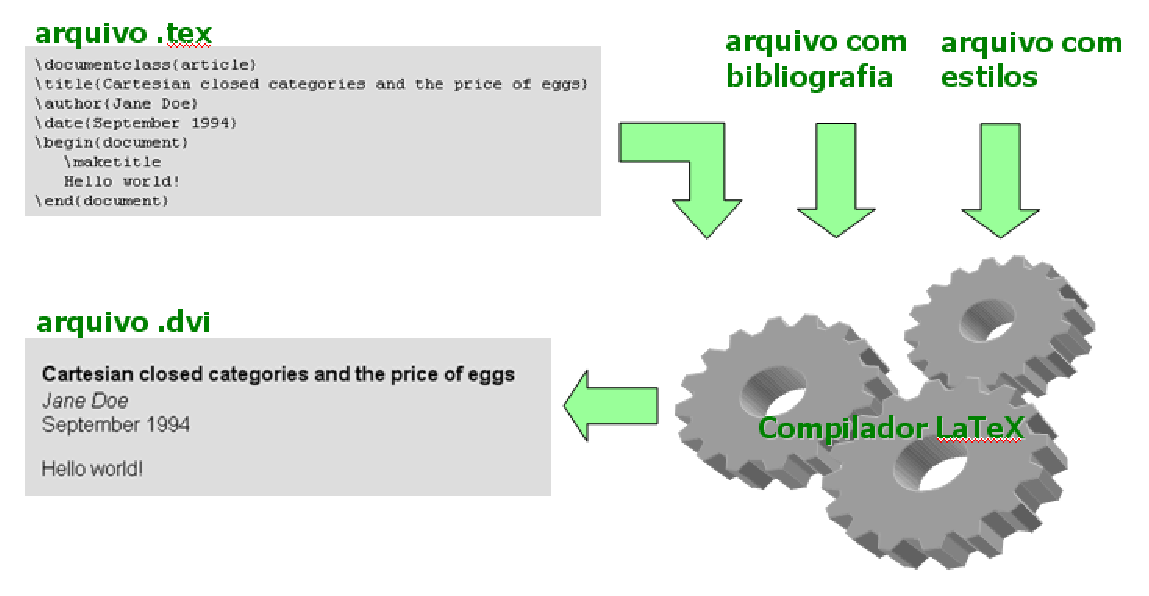
\includegraphics{figs/figuraTeste}}
   \end{center}
   \caption{Testando uma figura...\label{figuraEPS}}
\end{figure}


\subsection{Bla blá}

Uma subseção...

\subsubsection{ABC}

Uma subsub-seção.
         % Editar o arquivo introducao.tex
\chapter{Nome do Capítulo A}

Este capítulo apresenta um levantamento do estado da arte em armazenamento de documentos XML. Existem várias propostas na literatura blabla...

\begin{table}
\caption{Comparação dos trabalhos\label{tabela}} %título de tabelas sempre aparecem antes da tabela
\center{
\begin{tabular}{l|l}
\hline
Titulo Coluna 1   & Título Coluna 2\\
\hline
X                 & Y\\
X                 & W\\
\hline
\end{tabular}}
\end{table}

Os trabalhos blablabla são comparados na Tabela \ref{tabela}. 
          % Editar o arquivo capituloA.tex
\chapter{Nome do Capítulo B}

O capítulo...
          % Editar o arquivo capituloB.tex
\chapter{Conclusão}

Este trabalho mostrou...

As principais contribuições deste trabalho são...
          % Editar o arquivo introducao.tex

\bibliography{post-text/referencias}          % Editar o arquivo "referencias.bib"
\bibliographystyle{latex-stuff/abnt-ufrgs}      % Procura pelo arquivo "abnt-ufrgs" - normas ABNT.

\clearpage

\appendix
%Obs.: No sistema operacional Windows, ao modificar este arquivo usando WinEdt, pode gerar erro do tipo:

%Error: Unicode char \u8: not set up for use with LaTeX.

%Se esse erro acontecer no WinEdt, modifique o Apêndice no Texmaker, rode nele e depois no WinEdt.


% Se não tiver Apêndice, deixar este arquivo em branco.

\chapter{}

Escrever no Apêndice A

\clearpage

\chapter{}

Escrever no Apêndice B

\clearpage

\chapter{}

Escrever no Apêndice C

(...)
          % Editar o arquivo apendice.tex

\end{document}

%\citep* - citação completa, com todos os autores

%\citeyearpar - cita somente o ano da publicação
